% Template article for preprint document class `elsart'
% SP 2006/04/26

\documentclass{elsart}

% Use the option doublespacing or reviewcopy to obtain double line spacing
% \documentclass[doublespacing]{elsart}

% if you use PostScript figures in your article
% use the graphics package for simple commands
% \usepackage{graphics}
% or use the graphicx package for more complicated commands
\usepackage{graphicx}
% or use the epsfig package if you prefer to use the old commands
% \usepackage{epsfig}

% The amssymb package provides various useful mathematical symbols
\usepackage{amssymb}
\usepackage{xspace}

\usepackage{listings}

\usepackage{hyperref}


% The lineno packages adds line numbers. Start line numbering with
% \begin{linenumbers}, end it with \end{linenumbers}. Or switch it on
% for the whole article with \linenumbers.
% \usepackage{lineno}

% \linenumbers

\def\lhcb {LHC{\em b\/}\xspace}
\def\dirac{DIRAC\xspace}
\def\atlas {ATLAS\xspace}
\def\lhc {LHC\xspace}
\def\ganga {\textsc{Ganga}\xspace}
\def\python {\textsc{Python}\xspace}
\def\root {\textsc{Root}\xspace}
\def\gaudi {\textsc{Gaudi}\xspace}
\def\athena {\textsc{Athena}\xspace}
\def\garfield {\textsc{Garfield}\xspace}
\def\diane {\textsc{DIANE}\xspace}
\def\grid {Grid\xspace}
\def\GPI{GPI\xspace}
\def\roofit{\textsc{RooFit}\xspace}
\newcommand{\code}[1]{\texttt{#1}}
\newcommand{\val}[1]{\emph{#1}}

\begin{document}

\begin{frontmatter}

% Title, authors and addresses

% use the thanksref command within \title, \author or \address for footnotes;
% use the corauthref command within \author for corresponding author footnotes;
% use the ead command for the email address,
% and the form \ead[url] for the home page:
% \title{Title\thanksref{label1}}
% \thanks[label1]{}
% \author{Name\corauthref{cor1}\thanksref{label2}}
% \ead{email address}
% \ead[url]{home page}
% \thanks[label2]{}
% \corauth[cor1]{}
% \address{Address\thanksref{label3}}
% \thanks[label3]{}

\title{Ganga -- a tool for computational-task management and easy access to \grid
  resources}


% use optional labels to link authors explicitly to addresses:
% \author[label1,label2]{}
% \address[label1]{}
% \address[label2]{}

\author[a:Cambridge]{Frederic Brochu}
\author[a:Imperial]{Ulrik Egede\corauthref{cor1}}
\corauth[cor1]{Corresponding author}
\ead{U.Egede@imperial.ac.uk}
\ead[url]{http://www.imperial.ac.uk/people/u.egede}
\author[a:Munich]{Johannes Elmsheuser}
\author[a:Cambridge]{Karl Harrison}
\author[a:Lancaster]{Roger Jones}
\author[a:CERN]{Hurng-Chun Lee\thanksref{HurngChun}}
\author[a:CERN]{Dietrich Liko}
\author[a:CERN]{Andrew Maier}
\author[a:CERN]{Jakub T. Mo{\'s}cicki}
\author[a:CERN]{Adrian Muraru}
\author[a:STFC]{Glenn Patrick}
\author[a:Imperial]{William Reece}
\author[a:Oxford]{Alexander Soroko}
\author[a:Birmingham]{Chun Lik Tan}

\address[a:Cambridge]{University of Cambridge, Cambridge, United Kingdom}
\address[a:Imperial]{Imperial College London, London, United Kingdom}
\address[a:Munich]{Ludwig-Maximilians-Universit\"{a}t, M\"{u}nchen, Germany}
\address[a:Lancaster]{Lancaster University, Lancaster, United Kingdom}
\address[a:CERN]{CERN, Geneva, Switzerland}
\address[a:STFC]{Science \& Technology Facilities Council, United Kingdom}
\address[a:Oxford]{University of Oxford, Oxford, United Kingdom}
\address[a:Birmingham]{University of Birmingham, Birmingham, United Kingdom}

\thanks[HurngChun]{On leave from Academia Sinica Grid Computing Centre (ASGC),
  Taiwan.}

\begin{abstract}
  We present the computational task-management tool \ganga which allows for
  the specification, submission, bookkeeping and post processing of
  computational tasks on a wide set of distributed resources.  \ganga
  effectively provides a homogeneous environment for processing data on
  inhomogeneous resources. We provide examples from High Energy Physics,
  demonstrating how an analysis can be developed on a local system and then
  transparently moved to a \grid system for processing of all available data.
  \ganga offers an API which can be used via an interactive interface, in
  scripts, or through a GUI. Specific knowledge about types of tasks or
  computational resources is provided at run-time through a plug-in system, 
  making new developments easy to integrate. We give an overview of the
  \ganga architecture, give examples of current use, and demonstrate how
  \ganga can be used in many different areas of science.
\end{abstract}

\begin{keyword}
Grid computing \sep Data mining \sep Task management \sep User interface
% keywords here, in the form: keyword \sep keyword

% 07. 	Instruments, apparatus, and components common to several branches of
%             physics and astronomy
% 07.05.Kf 	Data analysis: algorithms and implementation; data management
% 07.05.Wr 	Computer interfaces

% 29. 	Experimental methods and instrumentation for elementary-particle and
%             nuclear physics
% 29.50.+v 	Computer interfaces
% 29.85.+c 	Computer data analysis

% 87. 	Biological and medical physics
% 87.18.Bb 	Computer simulation

% 89. 	Other areas of applied and interdisciplinary physics
% 89.20.Ff 	Computer science and technology

% PACS codes here, in the form: \PACS code \sep code
  \PACS 07.05.Kf \sep 07.05.Wr \sep 29.50.+v \sep 29.85.+c \sep 87.18.Bb \sep
  89.20.Ff
\end{keyword}
\end{frontmatter}

% main text

\section{Introduction}
\label{sec:intro}
\ganga is an easy-to-use frontend for the configuration, execution, and
management of computational tasks. The implementation uses an object oriented
design in \python. It started as part of the GridPP
project~\cite{Faulkner:2006px} to serve as a \grid user interface for data
analysis within the \atlas~\cite{Armstrong:1994it} and
\lhcb~\cite{Amato:1998xt} experiments in High Energy Physics where large
communities of physicists need access to \grid resources for data mining
and simulation tasks.

\ganga provides an API which can be used either interactively at the \python
prompt, through a Graphical User Interface~(GUI) or programmatically in
scripts. The concept of a \emph{job} component is essential as it contains the
full description of a computational task, including: the code to execute; data
required for processing; data produced by the application; requirements on
processing environment; post-processing tasks; and meta-data for bookkeeping.
The purpose of \ganga can then be seen as making it easy for a user to create,
submit and monitor the progress of jobs. \ganga keeps track of all jobs and
their status through a repository that archives all information between
independent \ganga sessions. It is possible to switch between executing a job
on a local PC and on the \grid by changing a single parameter in a job. This
simplifies the progression from rapid prototyping on a local PC, to
small-scale tests on a local batch system, to an analysis of a large dataset
using \grid resources.

It is possible to make \ganga available to a user community with a high level
of customisation. For example, an expert within a field can implement a custom
application class describing a specific computational task. The class will
encapsulate all low-level configuration of the application, which is always
the same, and only expose a few parameters for configuration of a specific
task. The plug-in system provided in \ganga means that this expert
customisation will be integrated seamlessly with the core of \ganga at runtime,
and can be used by an end-user to process tasks in a way that requires
little knowledge about the interfaces of \grid systems. Issues such as
differences in data access between jobs executing locally and on the
\grid are similarly hidden.

\ganga has advantages over \grid Portals (see ~\cite{AHE,LEAD} for examples)
which allow users access to \grid functionality through their web browsers in
a simplified way. These portals are normally domain specific and allow users
of a distributed application to run it on the \grid without needing to know
much about \grid tools. While easy to use, a portal-based system is often too
restrictive.  In \ganga, the user has programmatic access through an API, and
has access to applications locally for quick turnaround during development. At
the same time \ganga may be used as a job management system integrated in a
larger system. In this case \ganga acts as a library for job submission and
control.

The implementation of \ganga follows an object oriented design and is
implemented in \python. \ganga is licensed under the GNU General Public
License\footnote{\ganga is licensed under GPL version 2 or any later version
  of your choice.}~\cite{GPL} and is available for download from
\url{http://www.cern.ch/ganga}. The installation of \ganga is trivial and
doesn't require any privileged access or server configuration as part of the
process. In the 9 month period following January 2007 \ganga has in total been
used at 83 domains around the world with 950 unique users running about 60k
\ganga sessions\footnote{The usage information is collected from a voluntary
  usage reporting system implemented in \ganga.}.

In this paper, we describe in section~\ref{sec:functionality} the overall
functionality, in section~\ref{sec:implementation} details of the
implementation, and in section~\ref{sec:mon} how the progress of jobs is
monitored. In sections~\ref{sec:useHEP} and~\ref{sec:other} we discuss how
\ganga is customised for specific user communities. In
appendix~\ref{sec:examples} we provide some examples of how the API in \ganga
can be used.

\section{Functionality}
\label{sec:functionality}
\ganga is a user-centric tool which allows easy interaction with heterogeneous
computational environments, configuration of the applications and coherent
organisation of jobs. \ganga functionalities may be accessed by a user with a
help of several interfaces: a text-based command line in \python, file-based
scripting and a graphical user interface~(GUI). This reflects different
working styles in different user communities and addresses various usage
scenarios such as using the GUI for training of new users, command line to
exploit advanced use-cases and scripting for automation of repetitive tasks.
For \ganga sessions the current usage is divided as (55\%, 40\%, 5\%) between
the interactive prompt, scripts and the GUI. As shown in
Fig.~\ref{fig:GPI_architecture} the three user interfaces are built on top of
the \ganga Public Interface~(\GPI) which in turn provides access to the \ganga
core implementation.
\begin{figure}[htbp]
  \centering
  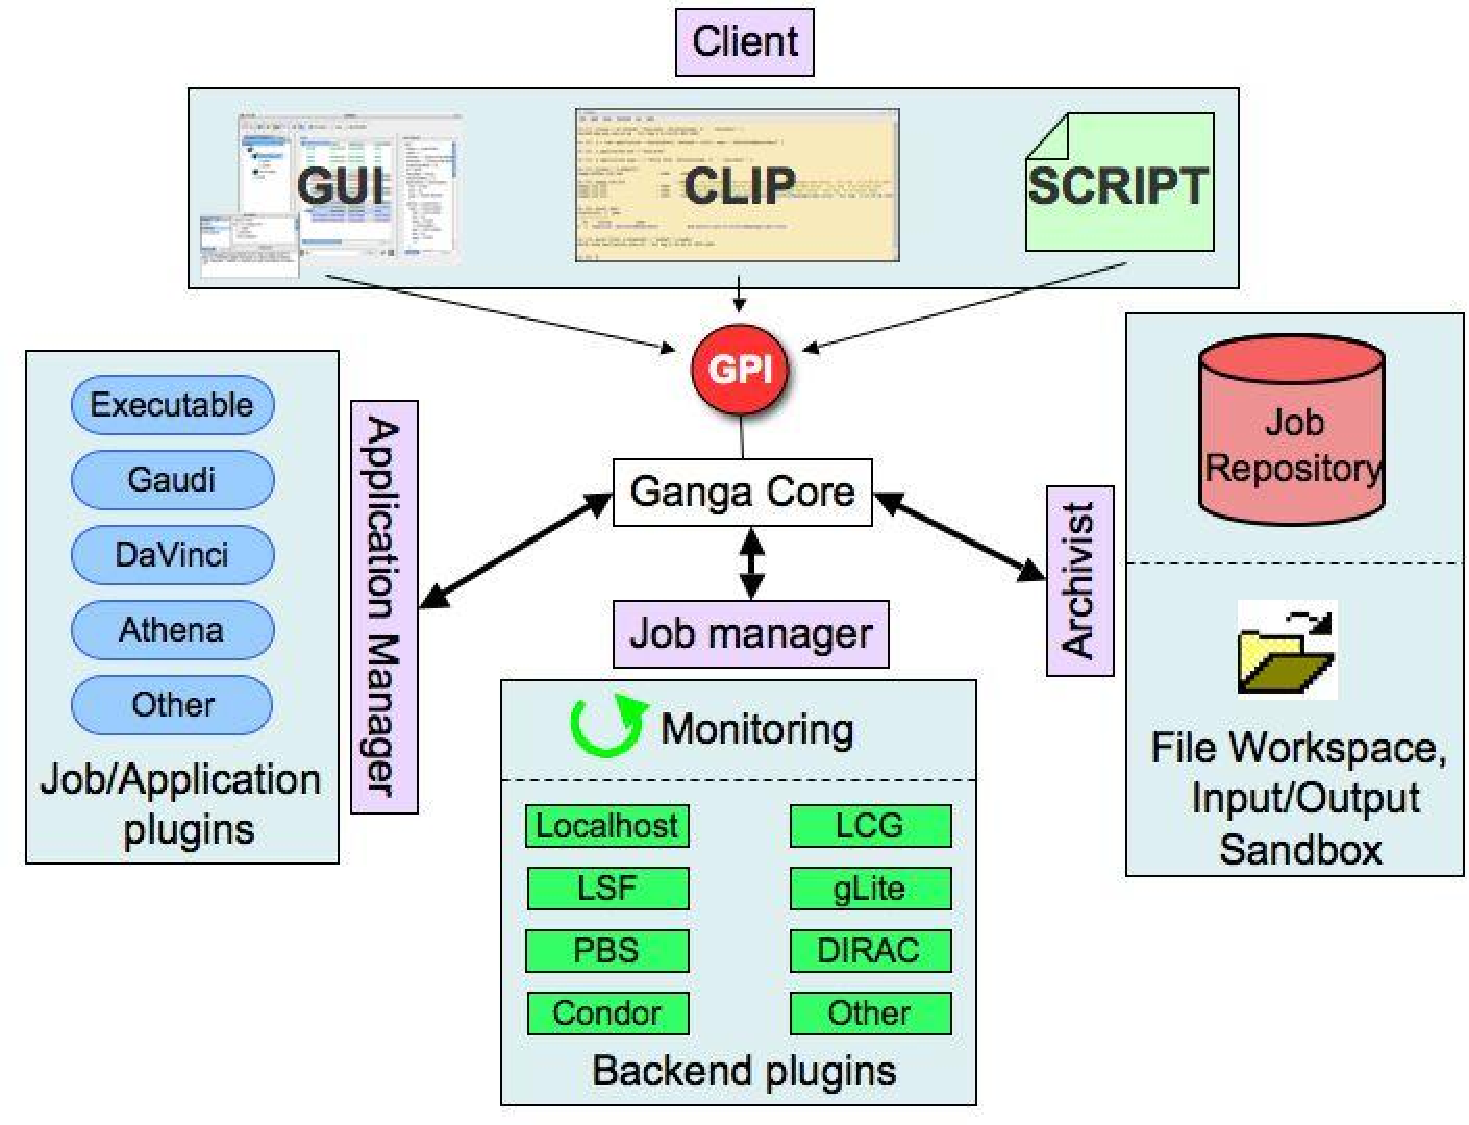
\includegraphics[width=14cm]{GangaOverview.pdf}
  \caption{The overall architecture of \ganga. The user interacts with the
    \ganga Public Interface via the GUI, the command line interface or
    scripts. Plug-ins are provided for different application types and
    backends where the applications can run. All jobs are persisted in the
    repository.}
  \label{fig:GPI_architecture}
\end{figure}

A job in \ganga is constructed from a set of components. All jobs are
required to have an application component and a backend component, which
define respectively the software to be run and the processing system to be
used.  Many jobs will also have input and output dataset components,
specifying data to be read and produced.  Finally, computationally intensive
jobs may have a splitter component, which provides a mechanism for dividing
into independent sub-jobs, and a merger component, which allows for the
aggregation of sub-job outputs. The overall component structure of a job is
illustrated in Fig.~\ref{fig:JobComponents}
\begin{figure}
  \centering
  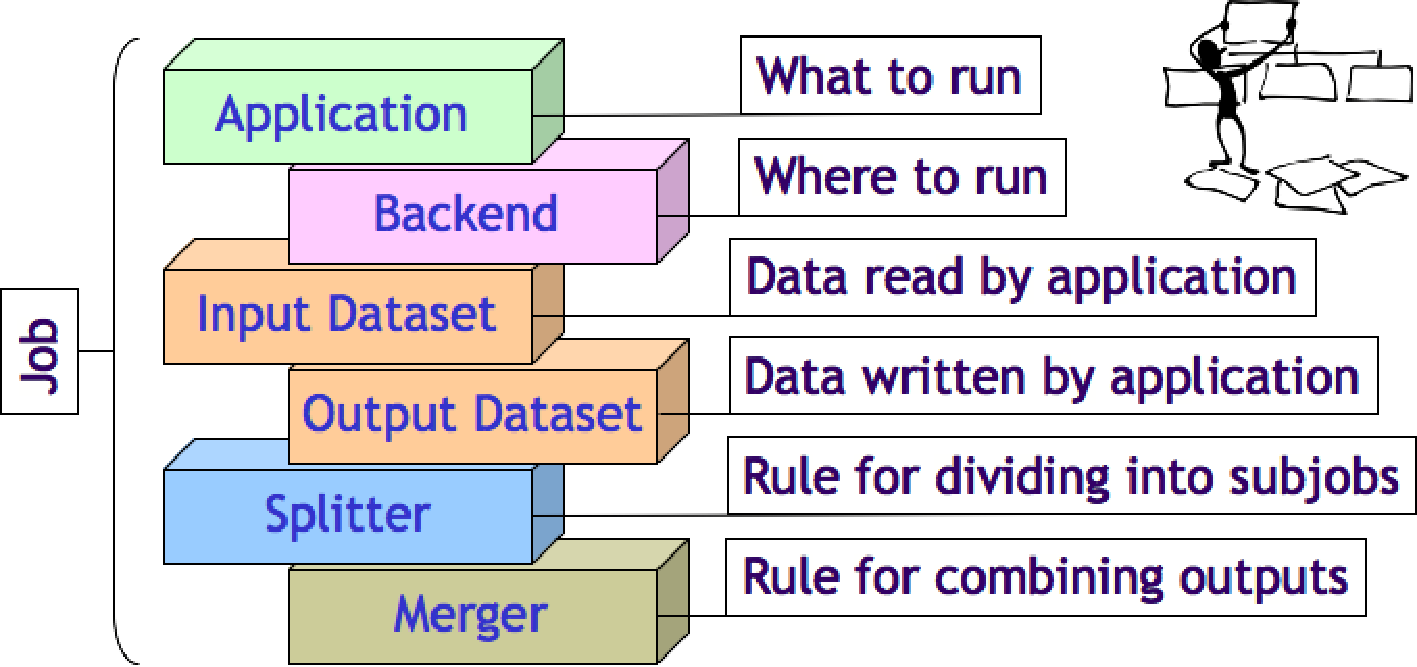
\includegraphics[width=14cm]{GangaJob.pdf}
  \caption{A set of components in \ganga can be combined to form a complete
    job. The application to run and the backend where it will run are
    mandatory while all other components are optional.}
  \label{fig:JobComponents}
\end{figure}

By default the \GPI exposes a simplified, top-level view suitable for most
users in their everyday work but at the same time allows for the details of
underlying systems to be exposed if needed. In Appendix~\ref{sec:examples}
examples are given of an actual interactive \ganga session using the \GPI.

After submitting a job \ganga takes over the control and a user may not modify
it, however a copy of the job may be easily created for subsequent
modification. \ganga monitors the evolution of submitted jobs and categorise
them into the simplified states \val{submitted},\val{running},
\val{completed}, \val{failed} or \val{killed}.

Other features of the \GPI allow frequently used job configurations to be
stored as \code{templates} and easily reused and labelling of jobs allow to
organise them in a hierarchical \code{jobtree}.

A large computational task may be split into a number of sub-jobs automatically
according to defined criteria and the output merged at a later stage. Each
sub-job will execute on its own and the merging of the output will take place
when they have all finalised.

All job objects are persisted in a job repository database whereas the input
and output files associated with the jobs are stored in a file workspace. Both
the repository and the workspace may be in a local filesystem or on remote
server.

For repetitive use-cases the \code{Robot} has been implemented. It is a \GPI
script which acts as a driver to periodically execute a series of
actions in the context of a \ganga session, where the actions are defined by
implementations of an action interface.  Without any coding, the driver can be
configured using existing action implementations to submit saved jobs, wait
for the jobs to complete, extract data about the jobs to an XML file, generate
plain text or HTML summary reports, and email the reports to interested
parties. Custom actions can easily be added by either extending or aggregating
the existing implementations or implementing the action interface directly,
allowing for a diverse variety of repetitive use-cases. See
section~\ref{sec:lhcb} for an example.

The framework does not force developers to support all combinations of
applications and backends but only the meaningful/interesting ones. To manage
this, the concept of a {\em submission handler} is introduced. The submission
handler is a connector between the application and backend components. At
submission time, it translates the internal representation of the application
into a representation accepted by a specific backend. This strategy allows
integration of inherently different backends and applications without forcing
a lowest-common-denominator interface.

Details of the different kinds of components are given below, along with
generic examples. More specialised components, designed for a particular
problem domain are considered in the sections dealing with use cases.

\subsection{Application components}
The application component describes the type of computational task to be
performed.  It allows characteristics and settings of some
%KUBA: we did not introduce the word schema before so I'd rather get rid of it here
piece of software to be defined, and provides methods specifying actions to be
taken before and after a job is processed.  The pre-processing (configuration)
step typically involves examination of the values set for the component
properties, and may require that these values be used to derive secondary
information.  For example, one of the properties might specify the path to a
file that needs to be read.  The post-processing step can be useful for
validation tasks.

The simplest application component (\texttt{Executable}) has three properties:
\begin{description}
\item[\code{exe :}] the path to an executable binary or script;
\item[\code{args:}] a list or arguments to be passed to the executable;
\item[\code{env :}] a dictionary of environment variables and the values they
  should be assigned before the executable is run.
\end{description}
The configuration method carries out integrity checks - for example
ensuring that a value has been assigned to the \code{exe} property.

\subsection{Backend components}
A backend component contains parameters describing the
behaviour of a processing system. The list of
parameters can vary significantly from one system to another, but can include,
%KUBA: consistency of usage of "parameters","properties" and "attributes" must be checked
for example, a queue name, a list of requested sites, the minimum memory
needed and the processing time required. In addition, some parameters carry the
information that the system reports back to the user, for example the 
system-specific job identifier and status, and the machine where a
job executed.

A backend component provides methods for submitting jobs, and for cancelling
jobs after submission, when this is needed.  It also provides methods for
updating information on job status, for retrieving output of completed jobs
and for examining files produced while a job is running.

Backend components have been implemented for a range of widely used processing
systems, including: local host, batch systems (PBS, LSF, SGE, and
Condor~\cite{Batch}), and \grid systems like gLite~\cite{LCG} and
ARC~\cite{NorduGrid}.  As an example, the batch backend component defines
a single property that may be set by the user:
\begin{description}
\item[\code{queue~~~~~~:}] Name of queue to which job should be submitted,
\end{description}
and defines three properties for storing system information:
\begin{description}
\item[\code{id~~~~~~~~~:}] job identifier;
\item[\code{status~~~~~:}] status as reported by batch system;
\item[\code{actualqueue:}] name of queue to which job has been submitted.
\end{description}

\subsection{Dataset components}
Dataset components generally define properties that uniquely identify a
particular collection of data, and provide methods for obtaining information
about it, for example its location and size. The details of how data
collections are described can vary significantly from one problem domain to
another, and the only generic dataset component in \ganga represents a null
(empty) dataset.  Other dataset components are specialised for use with a
particular application, and so are discussed later.

\subsection{Splitter components}
Splitter components allow the user to specify the number of subjobs to be
created, and the way in which subjobs differ from one another. As an example,
one splitter component (\code{ArgSplitter}) deals with executing the same task
many times over, but changing the arguments of the application executable each
time. It defines a single property:
\begin{description}
\item[args:] List of sets of arguments to be passed to an application.
\end{description}
Specialised splitters deal with creating subjobs that process different parts
of a dataset.

\subsection{Merger components}
Merger components deals with combining output of multiple jobs (subjobs). The
typical output are files containing data in a particular format, for example
text strings or data representing histograms. As examples, one merger
component (\code{FileMerger}) concatenates the files of standard output and
error returned by a set of subjobs, and another (\code{RootMerger}) sums
histograms produced in ROOT format~\cite{ROOT}.

Merging may be automatically performed in the background when \ganga retrieves
the job output or it may be controlled manually by the user.

\section{Implementation}
\label{sec:implementation}
In this section we provide details on the actual implementation of some of the
most important parts of \ganga.

\subsection{Components}
\label{sec:ComponentImplementation}
Job components are implemented as plug-in classes. They are imported by \ganga
at start-up if enabled in a user configuration file. In this way a given user
will only see the components that are relevant for their specific area of
work.

\begin{figure}
  \centering
  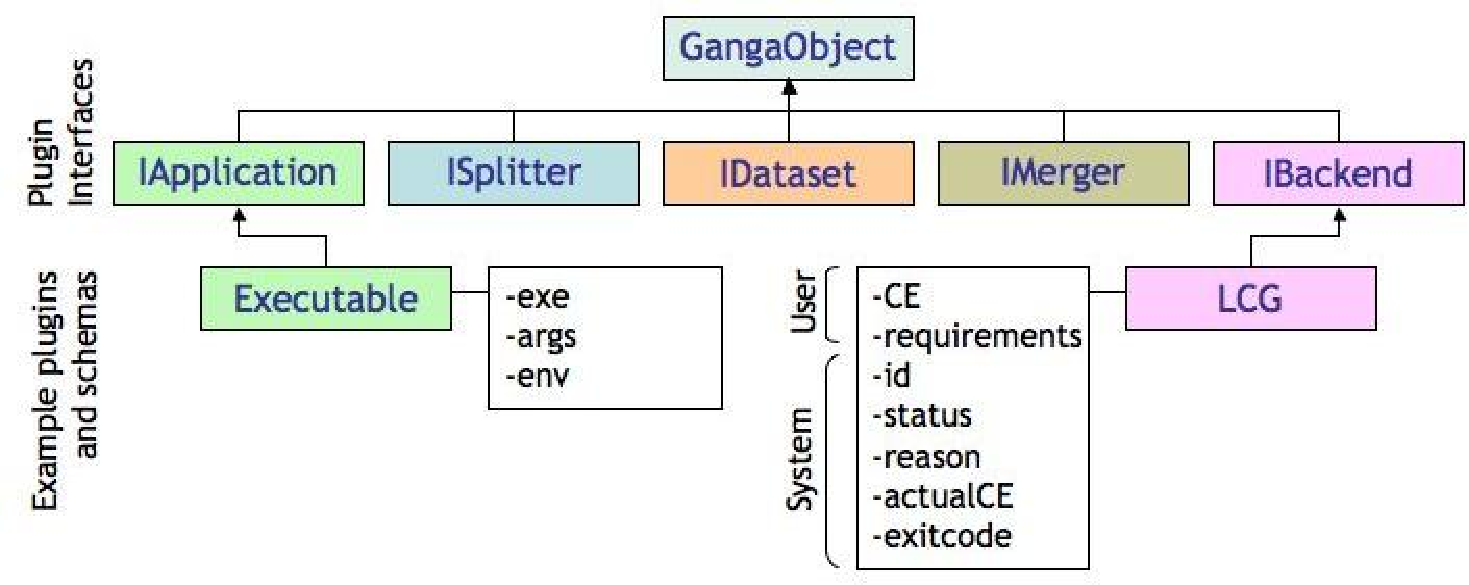
\includegraphics[width=14cm]{GangaPlugin.pdf}  
  \caption{A component class implements one of the abstract interfaces
    corresponding to the different parts of a job.}
  \label{fig:Components}
\end{figure}
Plugin development is simplified thanks to a set of internal interfaces and a
proxy generation mechanism. Component classes inherit from an interface class
as seen in Fig.~\ref{fig:Components}. Each plugin class defines a schema which
describes the plugin attributes and their properties such as the type
(read-only, read-write, internal), the visibility, user-convenience filters
and shortcuts.

The user do not interact with the plugin class directly but rather with an
automatically generated proxy class which is visible in the \GPI. The proxy
class only includes attributes defined as visible in the schema and methods
selected for export in the plugin class. The separation of the plugin and
proxy levels is very flexible. At the \GPI level the plugin implementation
details are not visible, all proxy classes follow the same design logic (for
example copy-by-value), persistency is automatic and the threading and session
level locking is transparent. In this way the low-level, internal API is
separated from the user-level \GPI.

\subsection{Job persistence}
\label{sec:persistence}
The \emph{job repository} provides job persistence in a simple database
assuring that any subsequent \ganga session have access to all previously
defined jobs. Once a job is defined in a \ganga session it is automatically
saved in the database. The repository provides a bookkeeping system that can
be used to select particular jobs according to job metadata. The metadata
includes such parameters as job name, type of application, type of submission
backend, and job status. It can be easily extended if required.

Currently \ganga supports both a local and a remote repository. In the local
repository the database is stored in the local file system thus providing a
standalone solution. The database code is implemented entirely in \python so
it is supported on any platform. For the remote repository the client relies
on the AMGA~\cite{AMGA} metadata server. The remote server supports secure
connections with user authentication and authorisation based on \grid proxy
certificates. The performance tests of both the local and remote repositories
show good scalability for up to 10 thousand jobs per user, with the average
time of individual job creation being about 0.2 second. There is scope for
further optimisation in this area by taking advantage of bulk operations and
on-demand job loading.

The job repository also includes a mechanism to support schema migration in
case of evolving plug-in components.

\subsection{Input and output files}

\ganga stores the job input and output files in a \emph{job workspace}. 
The current implementation use the local file system and has a simple
interface that allows transparent access to job sandbox files within the
\ganga framework. These files are automatically stored on a \emph{per job}
basis in a directory associated with the job, and a set of sub-directories is
used to separate specific parts of the job workspace like job input and output
and workspaces of subjobs.

User may access the files directly in the file-system or via simple commands
such as \texttt{job.peek()}. Internally \ganga handles the input and output
files using a simple abstraction layer which gives a possibility to replace
the implementation in a transparent way. A prototype using a
WebDav~\cite{WebDav} server demonstrated that all workspace data related to a
job can be accessed from different locations. In this case a local workspace
cache is still accessible via the normal file system.

A combination of remote workspace with the remote job repository effectively
creates a roaming profile where the same \ganga session can be accessed at
multiple locations in a way that is quite similar to what IMAP provides for an
email system.

\section{Monitoring}
\label{sec:mon}
\ganga provides two types of monitoring. One is the internal monitoring to
give the user information on the progress of jobs while the other is the
information connected with external monitoring services.

\subsection{Internal monitoring}
\label{sec:GangaMonitoring}
\ganga automatically keeps track of job status updates in the background.  The
job status monitoring mechanism has been specifically designed to cope with
varying backend response times and load capabilities. As seen in
Fig.~\ref{fig:job_status_monitoring_mechanism} each backend is polled in a
different thread taken from a thread pool and there is an efficient mechanism
to avoid deadlocks from slowly-responding backends. The poll rate may be
flexibly adjusted on per-backend basis.
\begin{figure}[htbp]
  \begin{center}
    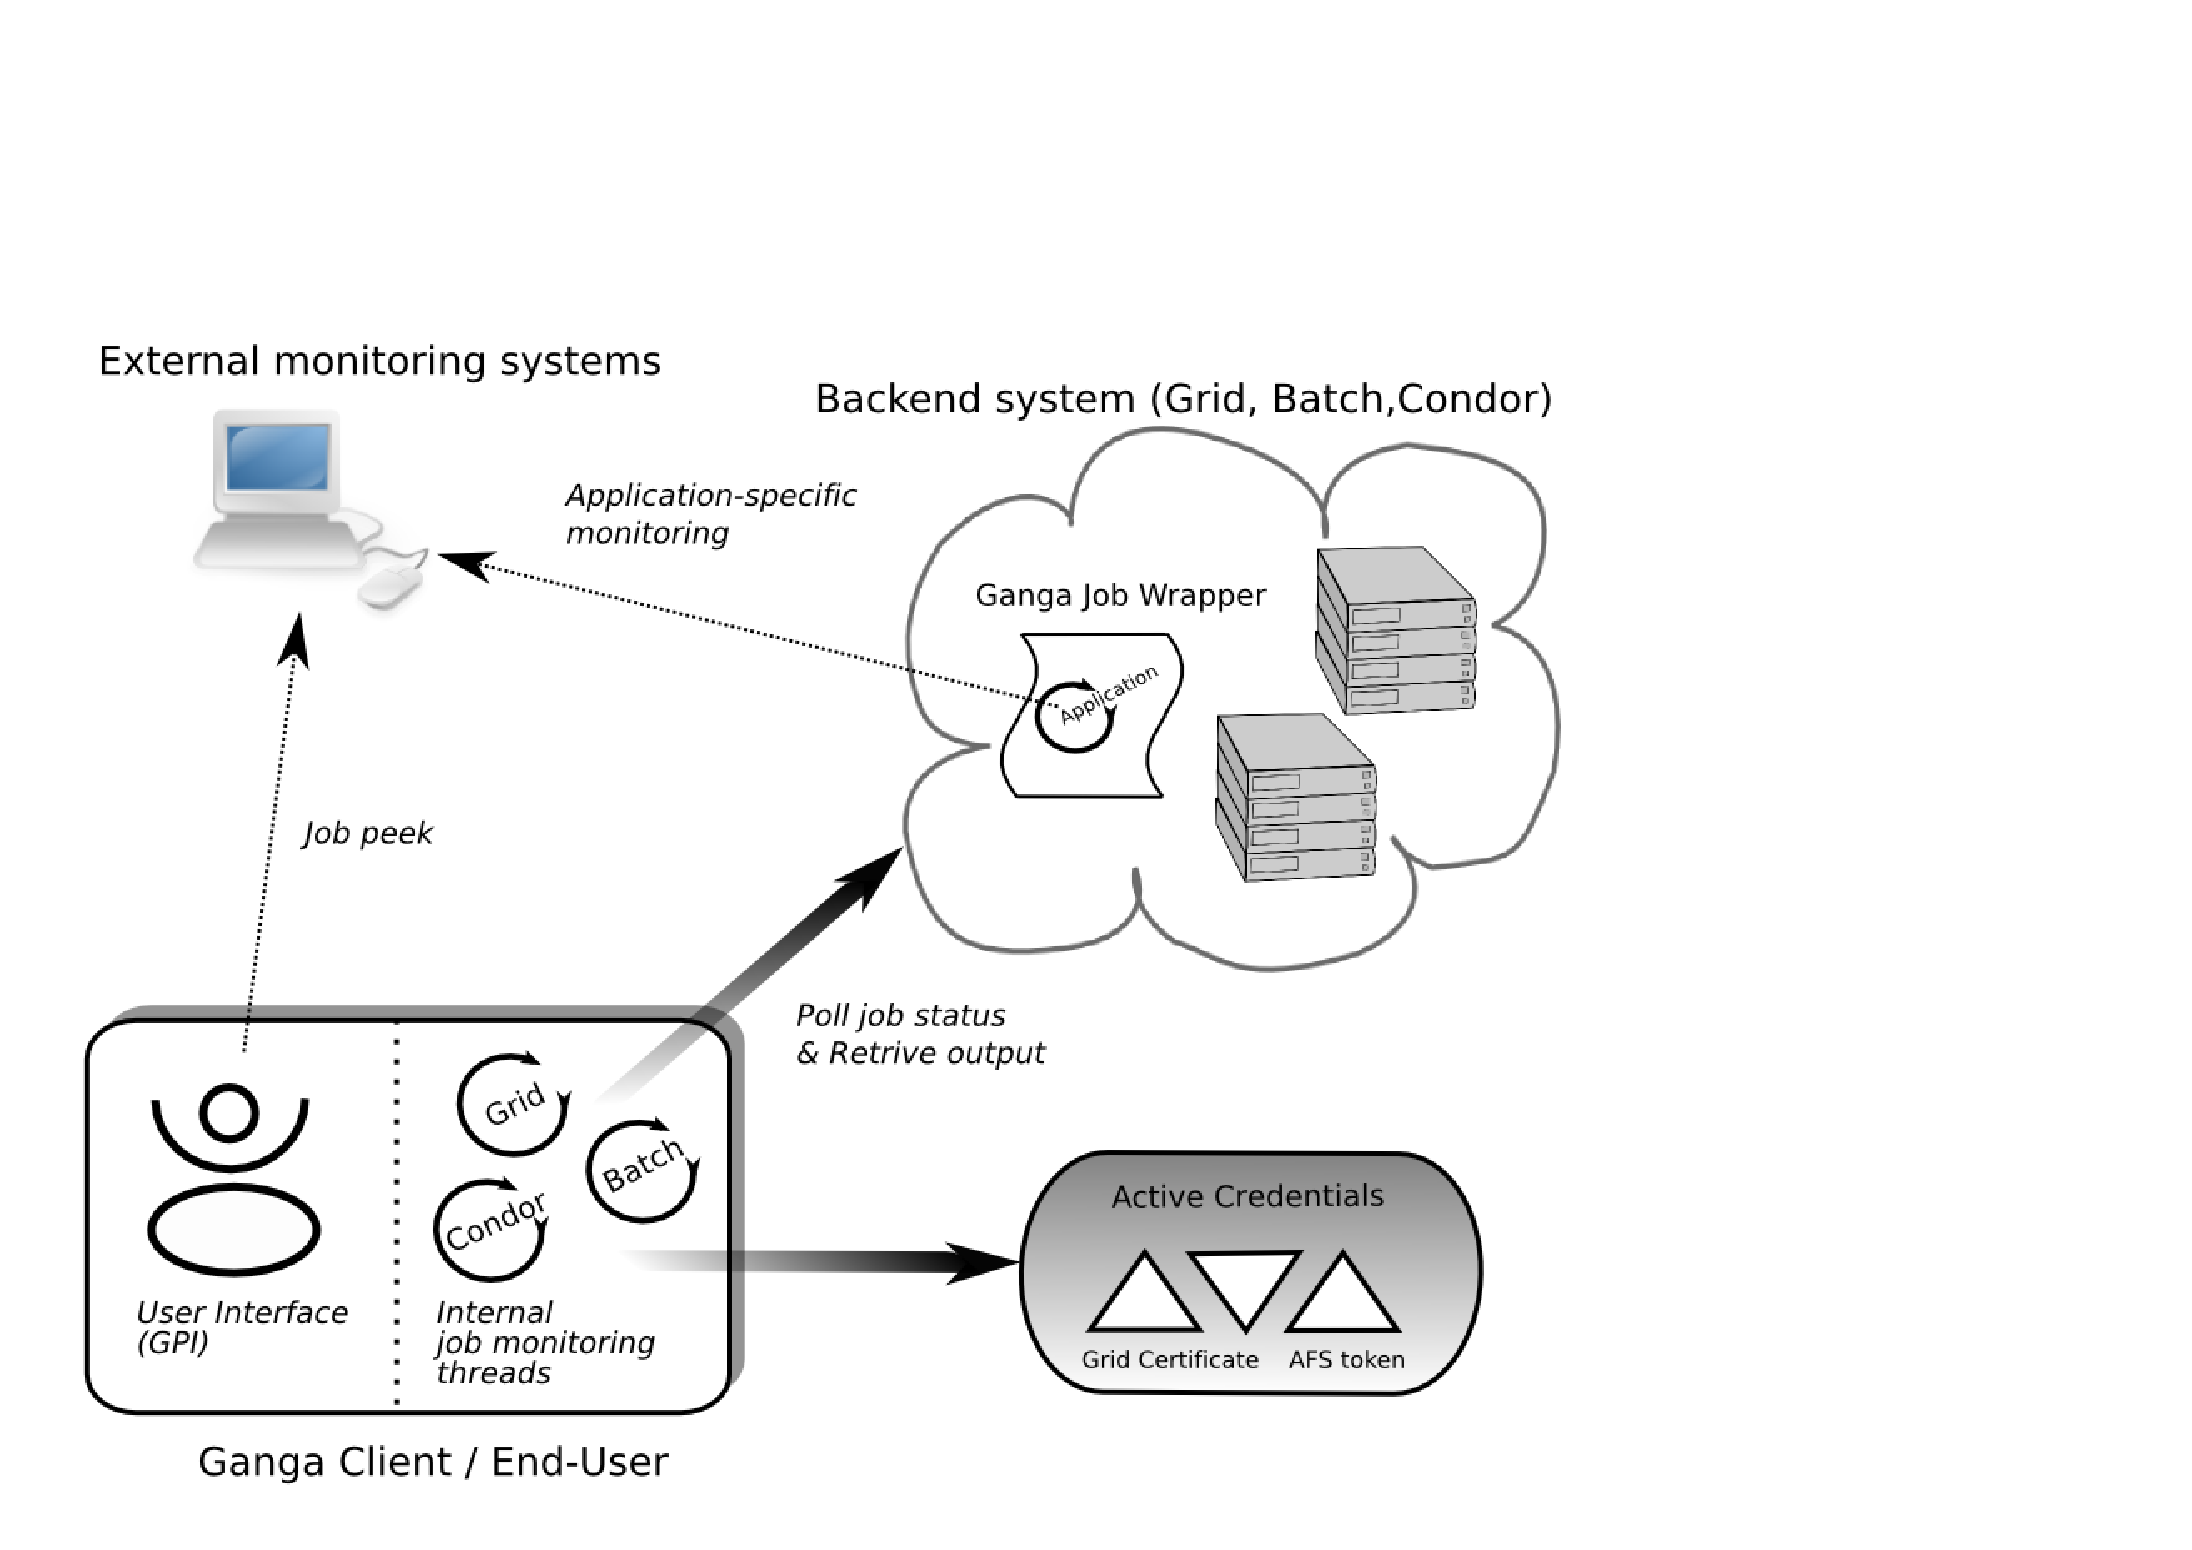
\includegraphics[width=1 \textwidth]{monitoring.pdf}
    \caption{The main monitoring thread takes care of checking for valid
      credentials, updating the table of jobs for each backend to monitor and
      feed the queue of updates. The thread pool subsequently pick tasks from
      the front of the queue.}
    \label{fig:job_status_monitoring_mechanism}
  \end{center}
\end{figure}

The monitoring sub-system also keeps track of the time remaining until
authentication credentials expire. Examples of these are proxy certificates
for interacting with the \grid, and kerberos tickets for interacting with a
file system. The user is notified that renewal is required and if no action is
taken, \ganga is placed in a safe state where errors will not occur due to
lack of authentication.

\subsection{External Monitoring}
\label{sec:ExternalMonitoring}
\ganga external monitoring provides a way to dynamically plug in third party
monitoring sensors in order to report different metrics during the execution
applications. 

The monitoring sensors can be inserted both on the client side - where \ganga
runs - and also on the remote environment (worker node) where the application
runs, allowing the user to follow the entire execution flow.  Monitoring
events are generated when the job is submitted, started, finished and
periodically while the job executes on the worker node.

Each application and execution component in \ganga can be configured to use a
different monitoring sensor allowing to send not only generic execution
information but also the instrumentation of the application code to report
specific data.

Currently there are two particular implementations of monitoring sensors. One
is the Atlas Dashboard application monitoring\footnote{See
  \url{http://dashb-atlas-job.cern.ch/dashboard/request.py/jobsummary}.}.
Another is a custom service which allows the \ganga user to peek the standard
output produced by the job in real-time on the \grid. The streaming is done on
request and must be activated by the user on a per-job basis.

\section{Use in High Energy Physics}
\label{sec:useHEP}

The aim of the \atlas and \lhcb experiments is to make discoveries about the
fundamental aspects of the Universe through production of new particles at the
energy frontier and precision measurements of particle decays. The experiments
are located at the Large Hadron Collider~(\lhc) at the European Laboratory for
Particle Physics~(CERN), Geneva. Both experiments require processing of data
volumes of the order of petabytes per year, and rely on computing resources
distributed across multiple locations. The data-processing applications,
including simulation, reconstruction and final analysis for the experiments,
are based on the \gaudi/\athena \code{C++}~\cite{gaudi} framework which
provides core services, such as message logging, data access, histogramming,
and a run-time configuration system. 

The data from the experiments will be distributed at computing facilities
around the world. Users performing data analysis need a random access
mechanism to allow rapid pre-filtering of data based on certain selection
criteria so as to identify data of specific interest.

The role of \ganga within \atlas and \lhcb is to act as the interface for data
analysis by a large number of individual physicists. \ganga also allows for
the easy exchange of jobs between users which otherwise can be dificult due to
the complex configuration of analysis jobs.

\subsection{The \lhcb experiment}
\label{sec:lhcb}
Here we describe the way in which \ganga interacts with the application and
backend plug-ins which are specific to \lhcb.

For a specific analysis a user normally supply shared libraries which are
loaded at run-time and replace default implementations in the \gaudi
framework.  The applications are driven by a configuration file, including the
directives of which libraries to load, the properties to be set, and a list of
input data expected and the output that will be created.

\ganga includes an application component for \gaudi-based applications to ease
the task of peforming an analysis. During the configuration stage, prior to
submission the application component:
\begin{itemize}
\item sets up the environment for the chosen application;
\item determines which shared libraries from a local user area are required to
  run the job;
\item parses the configuration file supplied including all its dependencies;
\item uses the information obtained from the configuration file to determine
  the input data required and the outputs the job will create;
\item registers the inputs and outputs with the submission backend.
\end{itemize}
The \gaudi application component thus allows for the configuration of the
\gaudi application in a simple way. The user only need to know the name and
version to run and then supply a configuration file.

As user code is often included in the application there is the potential for
introducing bugs causing runtime errors during job execution. The transparent
move in \ganga from a local to a \grid backend means that the debugging can be
performed locally with quick response time before launching a large scale
analysis on the \grid where the response time is longer.

To evaluate the expected performance of a given analysis there is also a large
usage of the \roofit framework for performing ensemble testing on simplified
Monte Carlo samples. These jobs require large amounts of processing but rely
on no input data and produce only very small amounts of output. Hence they are
very easy to deploy on the \grid using the generic \root application component
in \ganga.

Data analysis using \grid resources in \lhcb are routed through the
\dirac~\cite{DIRAC} workload management system~(WMS). \dirac is a pilot based
system where a small script is submitted to the \grid which checks for the
presence of required software, network connectivity, available memory etc.: If
all requirements are satisfied the application itself is pulled from the WMS
and started; If the requirements are not satisfied the pilot will simply
terminate and the WMS will send a new pilot to the \grid. The system thus
improves the reliability of the \grid system towards the user. A \dirac backend
component is included in \ganga to support submission of jobs to the \dirac
WMS. Internally this component is using the \python API of
\dirac~\cite{DIRACAPI}.  Further details of distributed analysis model in
\lhcb is described in~\cite{lhcb:2005jj}.

A specific \emph{splitter} has been implemented for \lhcb which can divide the
analysis of a large dataset into many smaller subjobs. During the splitting of
the dataset it is ensured that any data associated with a specific subjob is
available in its entirety at a given location on the \grid. This gives a
significant optimisation as no job will have to copy data across the WAN
before an analysis can start. To do this a specialised dataset component is
implemented for \lhcb which has the ability to query the \lhcb file catalogue
for the location of data replicas.

In the first half of 2007 a total of 10k user jobs has been successfully
executed through the \dirac system with a maximum of above 1000 simultaneous
jobs. With the \lhcb experiment receiving its first data during 2008 this
usage is expected to rise dramatically.

The \code{Robot} in \ganga is used within \lhcb for \emph{end-to-end} testing
of the distributed analysis model. On a daily basis it sets up a set of
typical complex analysis jobs. It then monitors the progress of the jobs and
the eventual results they produce. The overall success rate and time to obtain
the results is recorded and published on the web. An action within the
\code{Robot} monitors this information across many days in the past to produce
long-term trends in the \emph{end-to-end} stability of the system.

\subsection{The \atlas experiment}
\label{sec:atlas}
The distributed analysis model is based on the \atlas computing
model~\cite{bib:atlascompmod} which requires that data is distributed at
various computing sites and user jobs are sent to the data location based on
the availability of the data.

An analysis job at the \atlas experiment will typically consist of a \python
or shell script that configures and runs a user algorithm in the \athena
framework~\cite{bib:atlascompmod}, reads and writes event files and
fills histograms/n-tuples. More interactive analysis may be performed on
large datasets stored as n-tuples.

There are several scenarios relevant for a user analysis ranging from analysis
with fast response time and a high level of user interaction, to analysis with
long response times and a low level of user interaction. The former is well
matched by the parallel \root facility PROOF~\cite{ROOT} for interactive usage
and fast turn around times on a local computing cluster while \ganga matches
well the latter conditions.

Analysis jobs produce large amounts of data which is stored and subsequently
retrieved within the \grid environment. To support this, the Distributed Data
Management system DQ2~\cite{bib:atlasdq2} developed within \atlas; it provides
a set of services to move data between \grid-enabled computing facilities
whilst maintaining a series of databases to track these data movements.  The
vast amount of data is also grouped into datasets based on various criteria
(e.g.  physics characteristics, production batch run, etc.) for more efficient
query and retrieval.

\subsubsection{\atlas User Analysis}
A typical \atlas user analysis consists of an event selection algorithm
developed in the Athena software framework. Large amounts of data are skimmed
for events that meet certain selection criteria. The events of interest are
stored in files that in the DQ2 system are grouped together as datasets. Some
of the specific features are:
\begin{itemize}
\item During job submission the dataset is queried for in the DQ2 system for
  its file content and location.  The number of possible \grid sites is then
  restricted to the dataset locations.
\item A job can be divided into several sub-jobs based on the number of files
  in a dataset. Every sub-job processes an even amount of files of the full
  dataset.
\item The user output data can be saved in the DQ2 system. After the \athena
  programme has finished during the \grid job execution the user output data
  is stored on the close storage element of the site the job was running at
  and registered in DQ2.
\end{itemize}

In total 37k jobs have been successfully processed by \atlas users using
\ganga on the \grid in the first half of 2007.

\subsubsection{\atlas User Monte Carlo simulations}
A second example for a user task is a small scale Monte Carlo (MC) production
of a few ten thousand events. The \emph{AthenaMC} application component has
been developed to integrate software used in the official \atlas MC Production
System~\cite{bib:atlasprodsys}.  The component consist of a set of
configuration files for the three MC production steps for event generation,
simulation and reconstruction.

\section{Other usage areas}
\label{sec:other}
\ganga offers a flexible and extensible user interface which is used beyond
the original scope of the \atlas and \lhcb collaborations. Here we provide
details on just a few of the other projects that have made use of \ganga in
various ways.

\subsection{Commercial usage}
\label{sec:Imense}
Imense Ltd has implemented a new kind of image retrieval system based on
automated analysis and recognition of image content. It allows ordinary users
to intuitively search for pictures using text queries consisting of keywords
or short natural language sentences. Unlike other image search solutions, the
system does not rely on image annotations or metadata, and does not require an
initial example image or sketch to be supplied by the user. Instead, it
features a range of image processing and analysis modules which can
automatically recognise semantic image content and use this as the basis for
the image index. A diagram illustrating the process involved is shown in
Fig.~\ref{fig:camtologytech}.
\begin{figure}[htb]
  \begin{center}
    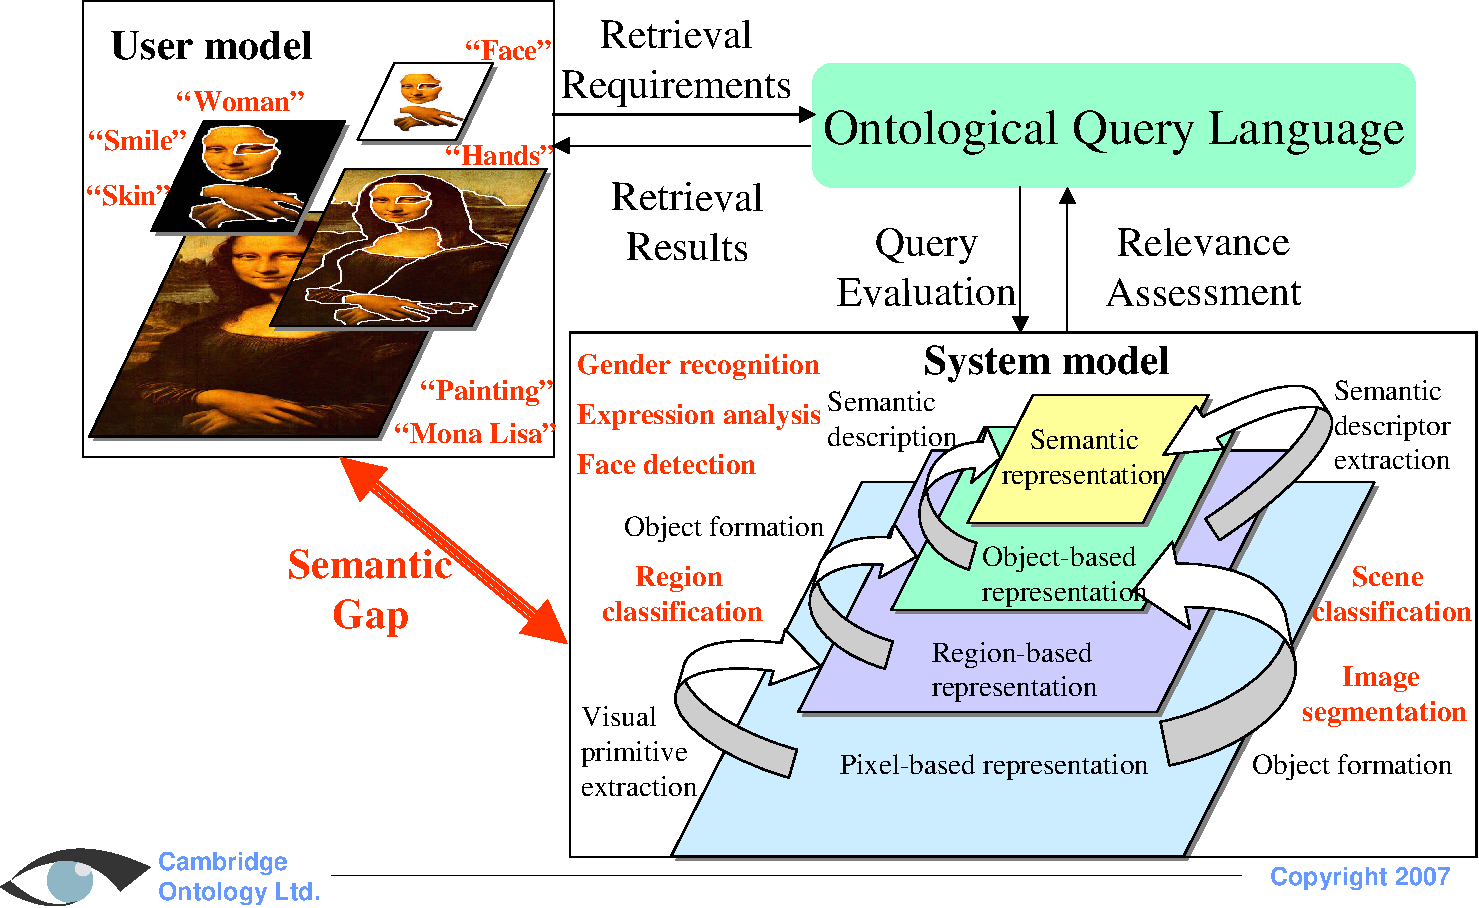
\includegraphics[width=0.85 \textwidth]{camtologyfigure.pdf}
  \end{center}
  \caption{Overview of the image analysis and recognition carried
    out by Imense Ltd.}
  \label{fig:camtologytech}
\end{figure}

By using the \ganga framework for job submission and management, it has been
possible to port and deploy a large part of Imense's image analysis technology
to the \grid to analyse the content of and build a searchable index over about
two million high resolution photographic images.

The processing stages involved in the image search system, i.e. image analysis
and indexing, are intrinsically sequential. In order to benefit from
parallelisation, it was decided to parallelise at the granularity of single
images or small subsets of images. Each image can therefore be processed in
isolation on the \grid, and such processing takes no more than a few seconds
or tens of seconds. In order to minimise overheads, several hundred images are
automatically agglomerated into a batch which is then submitted for processing
via \ganga, with the results of image processing and analysis being passed
back to the submission server upon successful completion.

Support for Imense has been added to \ganga through the implementation of two
specialised components: an application component that deals with running the
group's image-processing software, and a dataset component for taking care of
the output. Again the jobs can run both locally and on the \grid for maximal
flexibility.

At runtime, images are retrieved and segmented one at a time, all of the
images are classified, and finally an archive is created of the output files
(several per input image).  The archive is returned using the sandbox
mechanism in \ganga when using the \code{Local} backend, and is uploaded to a
storage element when using the \grid \code{LCG} backend.

The specialised dataset component provides methods for downloading a results
archive from a storage element, and for unpacking an archive to a destination
directory. These methods are invoked automatically by \ganga when an
image-processing job completes: the effect for the user is that a list of
images is submitted for processing and results are placed in the requested
output location indenpendent of the backend used.

\subsection{Small collaborations in High Energy Physics}
\label{sec:smallHEP}
Large user communities such as \atlas and \lhcb profit from encapsulating
shared use cases as specific applications in \ganga. At the same time
individual researchers or developers in the context of rapid prototyping
activities may resort to using generic application components such as
\code{Executable}. In such cases \ganga still provides the benefits of
bookkeeping and a programmatic access to job submission. For example a small
community of experts in the design of gaseous detectors such as drift chambers
use \ganga to run the \garfield~\cite{Garfield} simulation program on the
\grid.  A short \ganga script for submission of \garfield simulation jobs has
been developed. The submission script generates a chain of simulation jobs
using the \garfield generator of macro files and the \code{Executable}
application component.

The \garfield executables and a few small input files are placed directly into
the input sandbox of the job. The histogram and text output is returned in the
output sandbox. Such a simple approach allows to integrate certain
applications in just a few hours --- as it was the case for \garfield.

\subsection{\ganga interfaced to other frameworks}
\label{sec:GangaInOtherFrameworks}
The \ganga Public Interface is a backend and application neutral job
submission and management API. Therefore \ganga may be programmatically
interfaced to other frameworks and used as a convenient abstraction layer for
job management. \ganga combined with \diane, a lightweight agent-based
scheduling layer on top of the \grid~\cite{DIANE}, has been used in a number
of scientific activities such as: Monte Carlo simulation for dosimetric
studies in medical physics, statistical regresion testing of Geant 4 software
with a large number of \grid jobs; in-silico molecular docking in the search
of the potential drug candidates for Avian Flu~\cite{AvianFlu};
telecommunication applications; and computational-chemistry workflows. The
\diane worker agents are executed as \ganga jobs and thus the usage of the
resources may be controlled by the user from the \ganga interface. This
approach allowes to combine the efficiency of overlay scheduling systems such
as \diane with the well structured job management offered by \ganga as well as
combining \grid and non-\grid resources under a uniform interface.

\begin{figure}
  \centering
  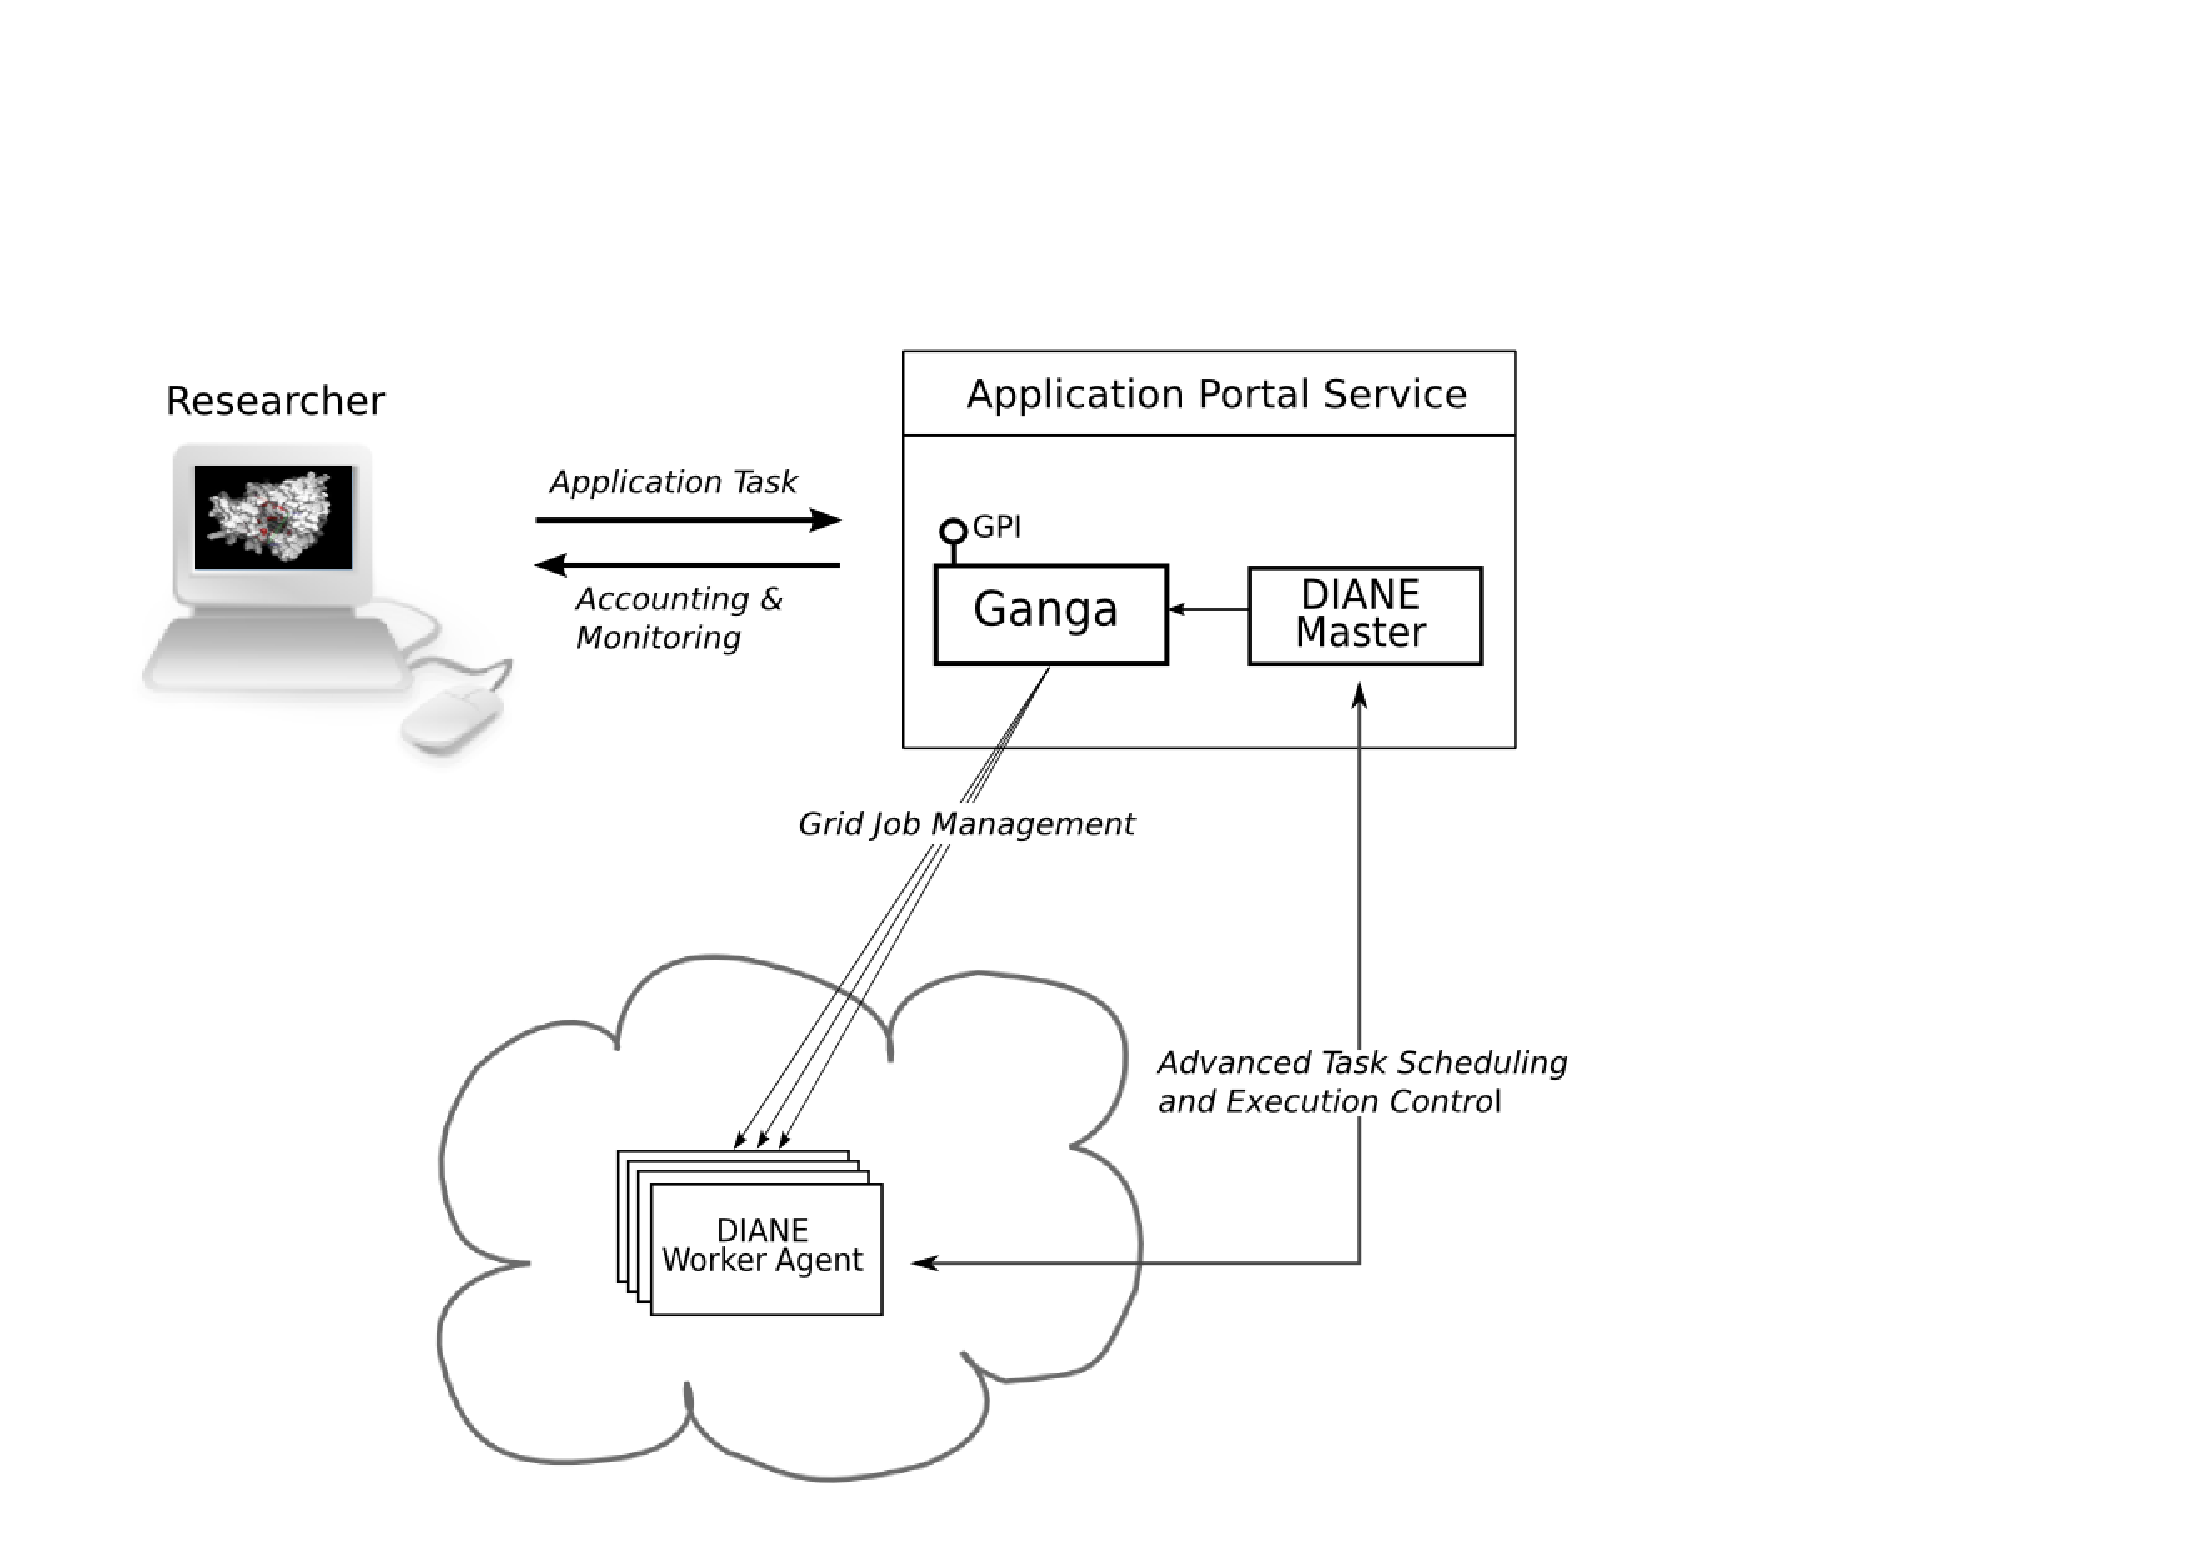
\includegraphics[width=1 \textwidth]{ganga-diane-portal.pdf}
  \caption{Ganga as a job management component embedded in DIANE and
    application portal frameworks.}
  \label{fig:webportal}
\end{figure}
%KUBA: text updated, figure not yet, it will be replaced by a schematic
%KUBA: diagram of portal/ganga/diane
\ganga may be flexibly embedded in web-based services such as the
bio-informatics portal developed by ASGC, Taipei. The portal is fully
customized for avian flu drug analysis.  The portal engine simply delegates
the job management to the embedded \diane/\ganga framework as shown in
Fig.~\ref{fig:webportal}. Powered by this job management approach, users can
also switch or combine the usage of heterogeneous computing environments (e.g.
\grid or local cluster) easily through the same web interface.

\section{Conclusion}
\label{sec:conclusion}
We have presented \ganga as a tool for managing jobs in an environment of
heterogeneous resources. In an easy way it is possible to define a
computational task which firsth can be executed locally for debugging and
subsequently to the \grid for large scale data mining. We have shown how \ganga
will aid the task specification, take care of job submission, monitoring and
output retrieval and provide an intuitive bookkeeping system.

We have demonstrated the advantages of having a well defined API which can be
used either interactively at the \python prompt, through a GUI or
programmatically in scripts. \ganga is easy to extend to become a specialised
interface for a new area of science through the plugin system for new
components. We have provided examples of the use of \ganga from within High
Energy Physics, medical physics and image processing.

\ganga has a large user base, is in active development and has adevelopment
team which is keen to provide initial support for new scientific or commercial
projects which would be interested in using \ganga.

\section{Acknowledgements}
\label{sec:acknowledgements}
The development of \ganga has partially been funded by GridPP under grants
from the research councils PPARC and STFC in the United Kingdom. \ganga makes
use of results produced by the Enabling Grids for E-sciencE project, a project
co-funded by the European Commission (under contract number INFSO-RI-031688)
through the Sixth Framework Programme~\cite{EGEE}.

The developers would also like to thanks the large base of users from both
within and outside High energy Physics for their mutiple suggestions for
improving \ganga and their help in debugging problems.


% The Appendices part is started with the command \appendix;
% appendix sections are then done as normal sections
% \appendix
\appendix

\section{Examples}
\label{sec:examples}
Below we give a set of examples of working with \ganga. For ease of reading,
\python keywords are in bold. First we look at a complete \ganga session
\vspace{-2ex}

\tiny
\lstset{language=Python} \lstset{commentstyle=\textit}
%\lstset{labelstep=1}
%\lstset{backgroundcolor=,framerulecolor=}
\lstset{backgroundcolor=,rulecolor=}
%\begin{lstlisting}[frame=tb,escapechar=!]{}
\begin{lstlisting}[escapechar=!]{}
!
\begin{verbatim}
~ % ganga
*** Welcome to Ganga ***
Version: Ganga-4-4-2
Documentation and support: http://cern.ch/ganga
Type help() or help('index') for online help.

This is free software (GPL), and you are welcome to redistribute
it under certain conditions; type license() for details.
\end{verbatim}!
[1]: j=Job(name='MyJob')      # Create a default job
[2]: j.submit()               # Submit the job

# wait for the monitoring

[3]: j.peek('stdout')         # Look at the output
[4]: j=j.copy(name='GridJob') # Make a copy of the job
[5]: j.backend=LCG()          # Change backend to the Grid
[6]: j.submit()               # Submit the job
[7]: jobs                     # List jobs
!
\begin{verbatim}
Job listing
\end{verbatim}!
[8]: ^D                       # Quit Ganga.
\end{lstlisting}
\normalsize

\vspace{-2ex}
In the next example we will create a more complex job for analysis of \lhcb
data. A splitter will be used to divide the analysis into a set of shorter
jobs. Data is assigned though logical identifiers and the \dirac WMS will then
sort out to send the job to one of the locations having the data available.
\tiny
\begin{lstlisting}[escapechar=!]{}
[1]: j=Job(application=DaVinci(),backend=Dirac())
[2]: j.inputdata=LHCbDataset(files=[  # Data to read
...      'LFN:/foo.dst',
...      'LFN:/bar.dst',
...      many more data files])
[3]: j.splitter=DiracSplitter()       # We want subjobs
[4]: j.submit()
!
\begin{verbatim}
Job submission output
\end{verbatim}!
\end{lstlisting}
\normalsize

\vspace{-2ex}
We can also use the interactive prompt together with standard \python syntax.
Here we print the status of the subjobs created above as well as the location
where they ran.
\tiny
\begin{lstlisting}[escapechar=!]{}
# Status of jobs and where they ran
[5]: for subjob in j.subjobs: 
...       print subjob.status, subjob.actualCE
!
\begin{verbatim}
42
\end{verbatim}!
# Find backend identifier of all failed jobs
[6]: for j in jobs.select(status='failed'):
...       print j.backend.id
!
\begin{verbatim}
42
\end{verbatim}!
\end{lstlisting}
\normalsize

\vspace{-2ex}
Finally we provide a view of the graphical user interface. The overview of jobs
can be seen to the left, the details of an individual job to the right, and
partly overlaid the window for contructing a new job.

\begin{thebibliography}{00}

\bibitem{Faulkner:2006px}
  P.~J.~W.~Faulkner {\it et al.}  [GridPP Collaboration],
  %``GridPP: Development of the UK computing Grid for particle physics,''
  J.\ Phys.\ G {\bf 32} (2006) N1.
  %%CITATION = JPHGB,G32,N1;%%

\bibitem{Armstrong:1994it}
  W.~W.~Armstrong {\it et al.}  [ATLAS Collaboration],
  ``ATLAS: Technical proposal for a general-purpose p p experiment at the
  Large Hadron Collider at CERN'', CERN-LHCC-94-43.
  %%CITATION = CERN-LHCC-94-43;%%

\bibitem{Amato:1998xt}
  S.~Amato {\it et al.}  [LHCb Collaboration],
  ``LHCb technical proposal'', CERN-LHCC-98-004.
  %%CITATION = CERN-LHCC-P-4;%%
\bibitem{GPL} 
  The GNU General Public License,
  \url{http://www.gnu.org/licenses/gpl.html}.

\bibitem{AHE} 
  P.~ V.~Coveney {\it et al.}, ``The Application Hosting Environment:
  Lightweight Middleware for Grid-Based Computational Science'',
  Comp.~Phys.~Comm., {\bf 176} (2007), 406.

\bibitem{LEAD}
  Dennis Gannon {\it et al.}, ``The LEAD Science Portal Problem Solving
  Environment'', submitted to Conference on Interactive Information and
  Processing Systems for Meteorology, Oceanography, and Hydrology, 23rd, San
  Antonio, TX, 14-18 January 2007.

\bibitem{Batch}

  LSF \url{http://www.platform.com}, PBS \url{http://www.openpbs.org}, SGE
  \url{http://gridengine.sunsource.net}, Condor, D.~Thain, T.~Tannenbaum, and
  M.~Livny, ``Distributed Computing in Practice: The Condor Experience"
  Concurrency and Computation: Practice and Experience'', {\bf 17, 2-4}
  (2005), 323, \url{http://www.cs.wisc.edu/condor/}

\bibitem{LCG}
Worldwide LHC Computing Grid, \url{http://www.cern.ch/LHCgrid}.

\bibitem{NorduGrid} 
  M.~Ellert {\it et al.}, ``Advanced Resource Connector middleware for
  lightweight computational Grids'', Future Generation Computer Systems
  (2007) {\bf23}.
  
\bibitem{ROOT}
  Rene Brun and Fons Rademakers, ``ROOT - An Object Oriented Data Analysis
  Framework'', Proceedings AIHENP'96 Workshop, Lausanne, Sep. 1996, Nuclear
  Ins. Methods Phys. Res., {\bf A389} (1997) 81. See also
  \url{http://root.cern.ch}.

\bibitem{IPython} The enhanced interactive Python shell IPython.
  \url{http://ipython.scipy.org/}

\bibitem{AMGA} B.~Koblitz, N.~Santos and V.~Pose, ``The AMGA metadata
  Service'', to appear in Jour. of Grid Computing.

\bibitem{WebDav} WebDav is a set of extensions to the HTTP protocol which
  allows users to collaboratively edit and manage files on remote web servers.
  Specification in RFC4918. See also \url{http://www.webdav.org/}.

\bibitem{lhcb:2005jj}
    Antunes-Nobrega, R {\it et al.} [LHCb Collaboration],
  ``LHCb TDR computing technical design report'', CERN-LHCC-2005-019
  %%CITATION = CERN-LHCC-2005-019;%%

\bibitem{gaudi} 
  Gaudi provides the necessary interfaces and services for building HEP
  experiment frameworks in the domain of event data processing
  applications. \url{http://www.cern.ch/gaudi}.

\bibitem{DIRAC} 
  A.Tsaregorodtsev {\it et al.}, ``DIRAC, The LHCb Data Production and
  Distributed Analysis System'', Proceedings from CHEP06, 2006.

\bibitem{DIRACAPI} 
  S.~Paterson, ``LHCb Distributed Data Analysis on the Computing Grid'', Ph.D.
  Thesis, University of Glasgow, 2006 (CERN-THESIS-2006-053).

\bibitem{bib:atlascompmod}
  ATLAS Computing TDR, CERN-LHCC-2005-022.

\bibitem{bib:atlasdq2}
  ATLAS DQ2/DDM project wiki, 
  \url{https://twiki.cern.ch/twiki/bin/view/Atlas/DistributedDataManagement}.

\bibitem{bib:atlasprodsys}
  ATLAS Production System
  \url{https://twiki.cern.ch/twiki/bin/view/Atlas/ProdSys}.

\bibitem{Garfield} 
  The Garfield program for simulation of drift chambers.
  \url{http://www.cern.ch/garfield}

\bibitem{DIANE} J.~T.~Mo{\'s}cicki, ``Distributed analysis environment for
  HEP and interdisciplinary applications'', Nuclear Ins. Methods Phys. Res.,
  (2003) {\bf A502}, 426. See also
  \url{http://www.cern.ch/diane}.

\bibitem{AvianFlu}
  H.~C.~Lee {\it et al}, ``Grid-enabled high-throughput in silico screening
  against influenza A neuraminidase'', IEEE Trans Nanobioscience (2006), 
  {\bf 5(4)}, 288, doi:10.1109/TNB.2006.887943.

\bibitem{EGEE} 
  EGEE brings together 91 partners in 32 countries to provide a seamless Grid
  infrastructure available to the European research community 24 hours a day.
  \url{http://www.eu-egee.org}.

%  C.~Germain-Renaud, C.~Loomis , J.~T.~Mo{\'s}cicki and R.~Texier,
%  ``Scheduling for Responsive Grids'', Jour. of Grid Computing, Springer, 
% DOI: 10.1007/s10723-007-9086-4

% Text of bibliographic item

% notes:
% \bibitem{label} \note

% subbibitems:
% \begin{subbibitems}{label}
% \bibitem{label1}
% \bibitem{label2}
% If there is a note, it should come last:
% \bibitem{label3} \note
% \end{subbibitems}

\end{thebibliography}

\end{document}

